\subsection{Mikrocontroller}
\label{subsec:Mikrocontroller}

Der Mikrocontroller ist das Gehirn der Maschine. Er muss in der Lage sein mit allen Komponenten auf der Platine zu kommunizieren, die Tasks zu verarbeiten und abzuhandeln. Der ATMega2560 übernimmt diese Aufgabe.


\paragraph{Schema}\mbox{}

Damit der Mikrocontroller funktionieren kann, sind folgende Funktionen implementiert:
\begin{itemize}
\item Erzeugung des System-Clocks mit 16Mhz mittels Quarz.
\item In-System-Program-Connector (ISP) für die Grundkonfiguration des Mikrocontrollers.
\item Abtrennung des ISP von der SPI-Leitung.
\item Reset-Button für Neustart des Mikrocontrollers.
\item Kontroll-Led für Spannung am Mikrocontroller.
\end{itemize}

\begin{figure}[H]
\center
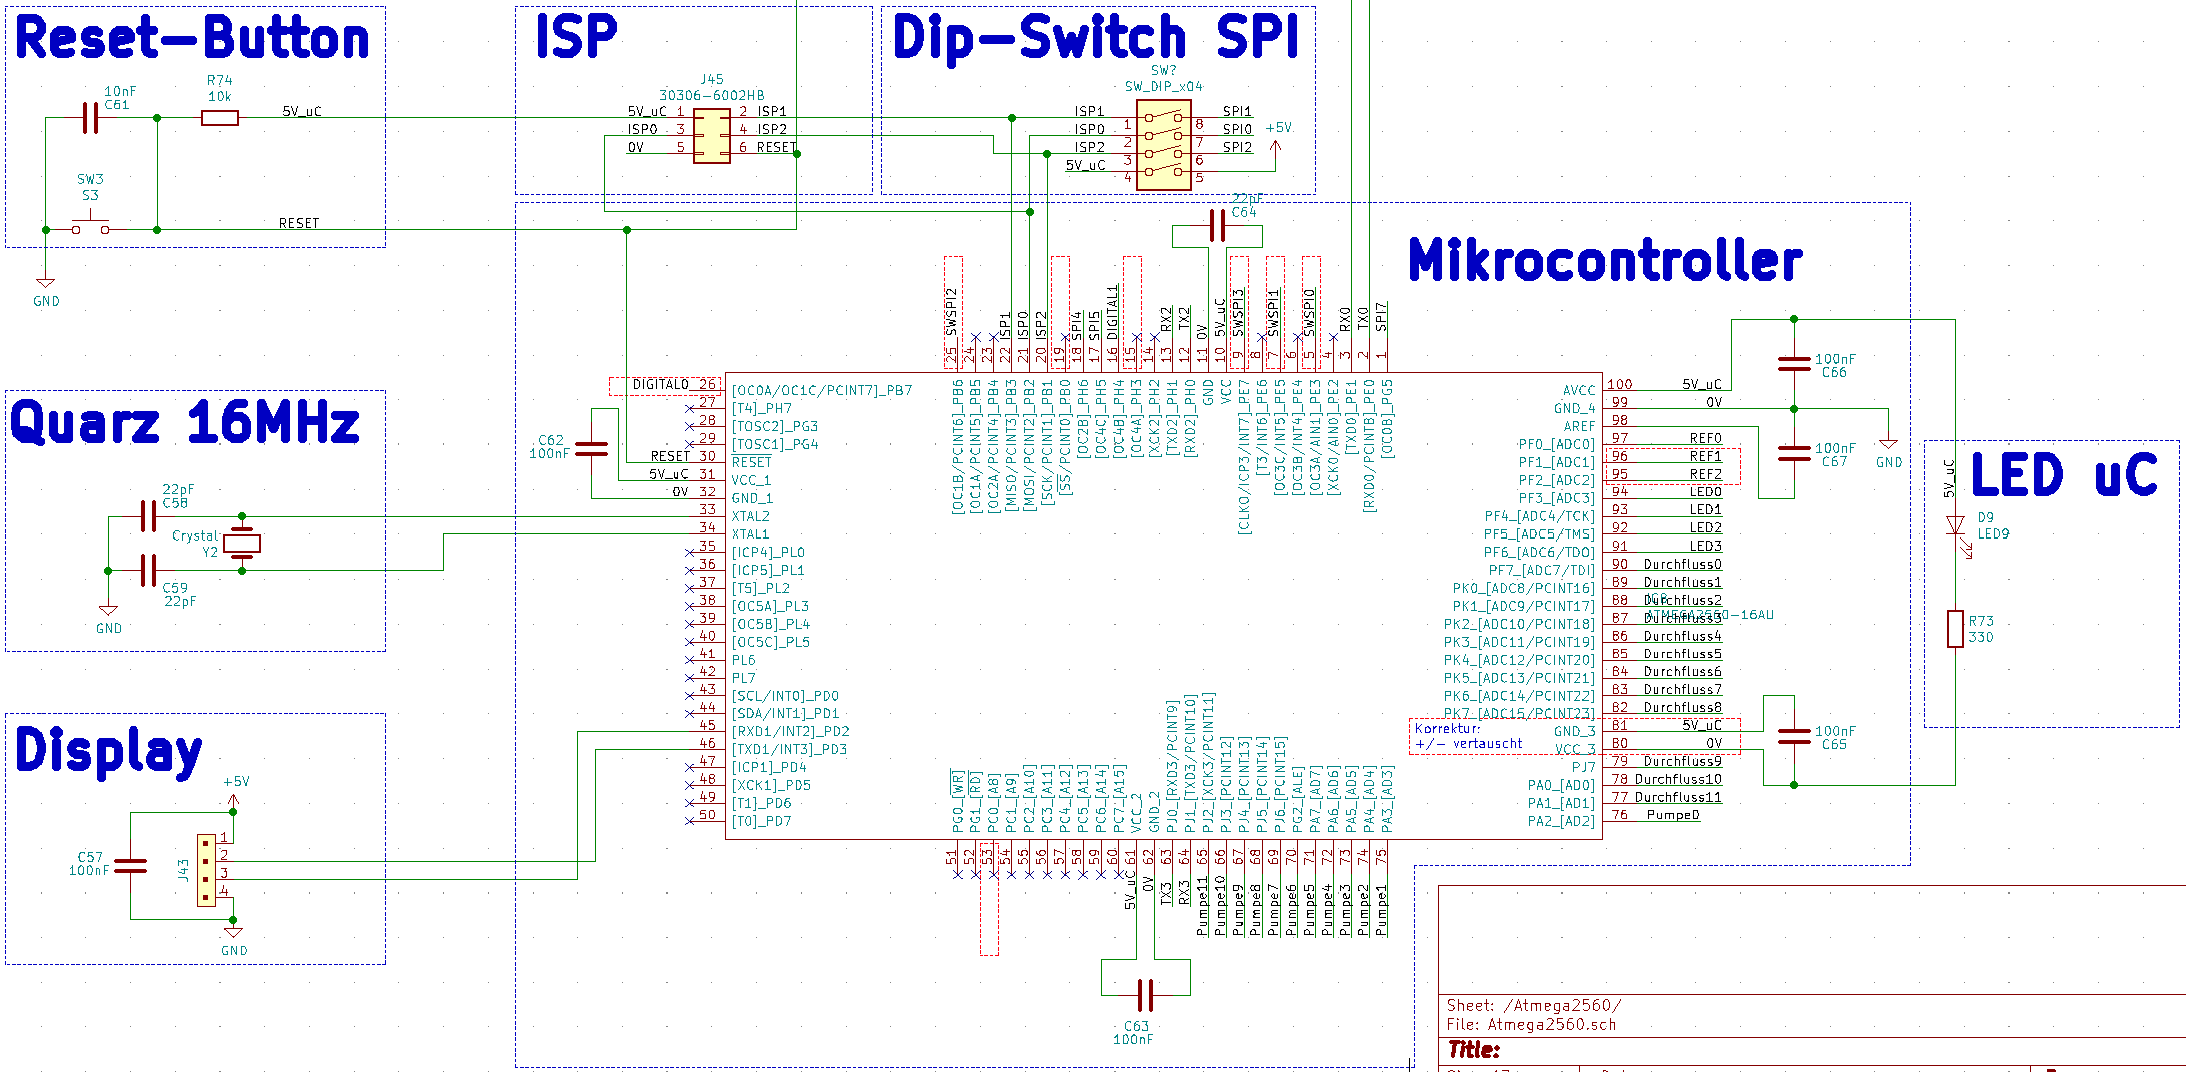
\includegraphics[width = \textwidth]{graphics/Schema_uC}
\caption{Schema Mikrocontroller}
\label{fig:Schema_uC}
\end{figure}

Die Korrekturen sind Rot im Schema in Abbildung \ref{fig:Schema_uC} eingezeichnet. Dazu gehören zum Ersten die zusätzlichen Software-SPI Pins für den FOC-Treiber, welche auf die Header-Pins des Wireless-/Bluetoothmodul DevKits führen und zum Zweiten das Umlegen der DIGITAL0-Leitung, welche die Enable-Leitung des Gate-Treibers darstellt. Weiter musste die Spannungsversorgung an einer Seite der Mikrocontrollers getauscht werden und zwei Leitungen für die Flüssigkeitsbeförderung umgelegt werden.

\paragraph{Funktionsbeschrieb der Schaltung}\mbox{}

Das Schema besteht aus dem Mikrocontroller IC8 mit den fünf Stützkondensatoren C62, bis C66 an den Spannungseingängen. Mit dem Full Swing Oscillator Crystal Y2 und den Kondensatoren C58 und C59 wird eine Frequenz von 16MHz generiert. Der Reset-Button SW3 dient dazu, den Mikrocontroller manuell neu zu starten. Der dazugehörige Kondensator C81 entprellt den Button und der Widerstand R74 zieht die Leitung mittels Pull-up auf VCC. Mittels dem ISP-Stecker kann über einen Programmer, z.B AVR MKII, auf den Mikrocontroller zugegriffen werden. Der DIP-Switch ist dazu da, die SPI-Leitungen von der ISP-Schnittstelle zu trennen. Die LED D9 gibt Auskunft ob Spannung am Mikrocontroller anliegt.

%Die Stützkondensatoren halten die Spannung am Mikrocontroller konstant. Die Quarz-Schaltung wird gebraucht, da der Mikrocontroller nur eine 8MHz-RC-Clock integriert hat, jedoch mit 16MHz gearbeitet wird. Der Reset-Button zieht in gedrücktem Zustand die Reset-Leitung auf GND. Dabei entlädt sich der Kondensator schnell, da er kurzgeschlossen wird. In offenem Zustand lädt sich der Kondensator C61 über den Widerstand R74 mit einer Zeitkonstante von $\tau = R_{74} \cdot C_{81} = 100us$. Die Trennung von SPI und ISP wird gemacht, sodass gewährleistet ist, dass bei der Inbetriebnahme des Mikrocontrollers die restlichen SPI-kommunikationsfähigen Komponenten nicht mitreden können. Zudem kann die 5V-Versorgungsspannung des Mikrocontroller vom Rest der Platine getrennt werden, sodass dieser auch bei ausgeschalteter Board versorgt werden kann, ohne die anderen Komponenten zu speisen. Deswegen auch die Betriebs-LED.